\section{Community Detection State of the Art}
\begin{figure}[h]
	\centering
	\includegraphics[width=0.6\linewidth]{0-resources/community1}
	\caption{An example of a communities structured graph. In it is well visible three community, enclosed by the rectangles. The image was made with Graphviz.}
	\label{fig:community1}
\end{figure}
The problem of community detection raises in many application scenarios from the necessity of finding groups of objects that have a large number of connections to each other. To represent problems where it is fundamental to empathize connection between objects, the graph theory is the main tool. A graph is a mathematical structure composed of nodes (or vertices) that denote the objects and edges (or links) that express some kind of relationship between objects and possibly having a weights that quantifies this relationship.
The Graph Theory born in 1736 when Euler used this mathematical abstraction to solve the puzzle of Königsberg’s bridges. Since then, this tool was used in several of Mathematics, Social, Biological and Technological application. In recent time, the approach to this studies has been revolutionized to deal with bigger and more complicated challenges, supported by the increasing computing power.
\begin{figure}[h]
	\centering
	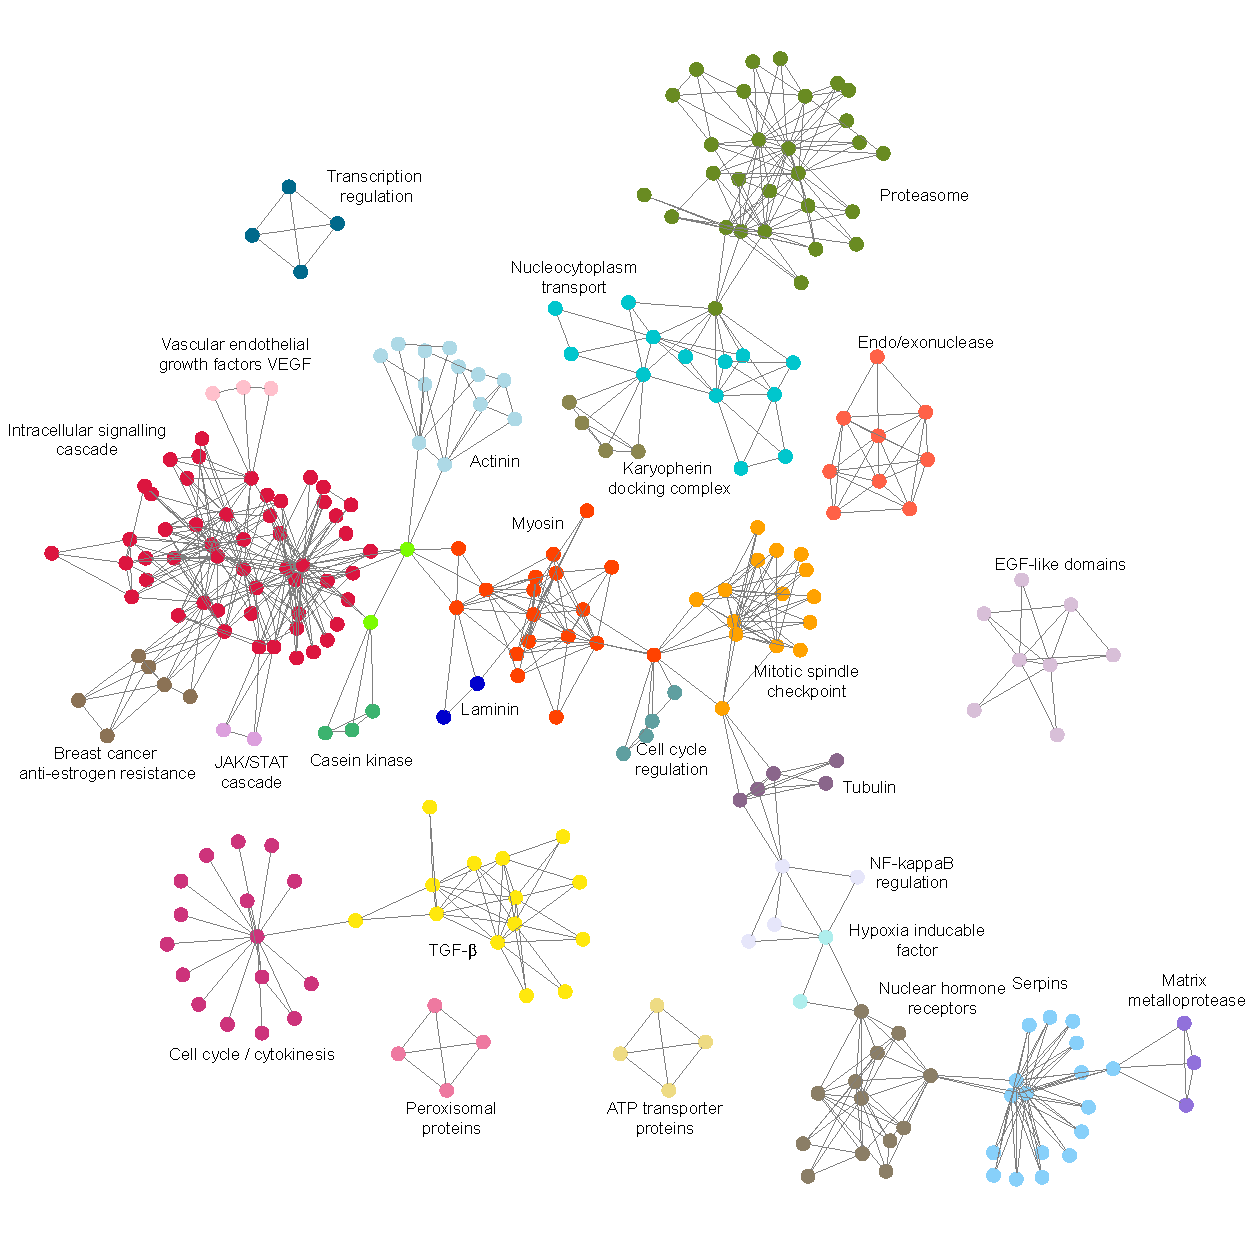
\includegraphics[width=1\linewidth]{0-resources/ppi}
	\caption{A protein protein iteration network of a rat cancerous cell. This image was reprinted from \cite{metastasis}.}
	\label{fig:ppi}
\end{figure}\\
The necessity of finding this high-connected substructure in graph arises from real problems of the previous field: for example, the study of Protein-Protein Interaction (PPI) networks is very important because the interaction between proteins is the basis of all process in the cell.\\ A study demonstrated that this type of network shown to be useful for highlighting key proteins involved in metastasis. \cite{metastasis} \\
Other examples can be found in the field of sociology: a historically well-know scenario is the Zachary's Karate Club. This dataset captures members of a Karate Club for 3 years.\cite{Zac77} An edge between two nodes represents an interaction between two members outside the club. At some point, a conflict between the administrator and a master led to split of the club into two separate groups. The question is if it is possible to infer who compose these two new groups basing on the information that this graph give to us. 
\begin{figure}
	\centering
	\includegraphics[width=0.6\linewidth]{0-resources/karateclub}
	\caption{Zacahry's karate club. \cite{Zac77} This image was made with Graphviz.}
	\label{fig:karateclub}
\end{figure}
This small network of 1977 is famous because it has often been used as a reference point to test the detection algorithms used to analyze huge social web networks.
In general this kind of problem, i.e. clustering people that belong to the same community base on interaction, it's useful not only in sociology but also in marketing: by knowing people with similar interests, it's possible to make better recommendation systems.\\
There are several of similar scenarios to apply this method in the real-world, all united by the fact that the data are unregular but it's present some well-defined topological structure that in a completely random graph are absent. A random graph is a fully disordered graph, firstly proposed by Erdös and Rényi \cite{random} in 1959: it's a graph where the probability that there is an edge between two nodes it's equal for all pairs of nodes and, for this reason, the degree of the nodes (i.e. the number of edges incident to a node) is homogeneous. In real networks, this is not true, because they are often scale-free (fallow a power-law distribution). An example of this is the study about the citations in scientific papers made by Derek J. de Solla Price in 1965 \cite{dsp} or the study about World Wide Web growing made by Albert-László Barabási et al in 1999 \cite{Barab}.
Furthermore, the degree distribution of the nodes is non-homogeneous not only globally but also locally, this due to the observation that there is a high concentration of edges within sets of nodes and a low concentration of edges between this sets. These two concepts are essential to formulate the formal definition of Community and Modularity. In this chapter will be presented some definitions of community and will be given an overview of some methods that are used to identify communities.
\subsection{Community Definitions}
The informal definition of community is there are many more edges inside the community versus the rest of the graph, but there isn't a unique quantitative definition of community. This kind of freedom is necessary because the concept of community is strictly connected to the problem that will be analyzed: for example, in some cases, it's necessary that community overlap, but in other problems, this is not necessary. There is a unique key constraint that allows talking about community detection: the graph must be sparse. A sparse graph is a graph where the number of nodes has the same magnitude of the number of edges. In the unweighted graph case, if the number of edges is far greater than the number of nodes, the distribution of edges among the nodes is too homogeneous for communities to make sense \cite{fortunato}. In that case, the problem nature is little different: we aren't interested anymore on the edge density between nodes but we have to use some kind of metrics (like similarity or distance) to clustering. In that case, the problem is more similar to data clustering. Despite this, assuming that a community is a subset of similar nodes it's reasonable, for this reasons some techniques (like spectral o hierarchical clustering) belonging to this field are adopted in community detection and will be shortly presented later on this thesis.
Following this, Fortunato \cite{fortunato} defines three main classes of community's definitions: \textit{local, global and based on vertex similarity}. Other types of definitions are still possible, but these three offers give a good summary of the problem. Now those classes will be presented to give an overview of the various approach that has been used to define this problem. 
\subsubsection{Local definitions}\label{local-def}
Considering that a community has a lot of interactions with the other nodes that are in it and few connections outside, it is fair to think about the communities as autonomous objects.
The local definitions are based on this concept. Directly from this concept, we can think at the community as a clique, i.e. a subset whose vertices are all adjacent to each other. This type of definitions it's too strict: even if just one edge is not present, the subset is not a clique, but the subset has a very high concentration of edges. For this reason, the clique definition is often relaxed, using, for example, $n$-clique, i.e. a subset in which all the vertices are connected by a path of length less than $n$.\\
Anyway, this type of definitions ensure that there is a strong cohesion between the nodes in the subset, but not ensure that there isn't a comparable cohesion between the subset and the rest of the graph. For this purpose, other definitions were proposed. 
Given a graph $G(V,E)$, the relative adjacency matrix $A$ and a subset of nodes $C$ where $C \in V$, we define the internal degree $k_v^{int}$ and the external degree $k_v^{ext}$ for each vertex $v$ that belongs to $C$ as the number of edges that connect the node $v$ with another node that belongs to $C$ and not belongs to $C$, respectively:
\begin{align}
k_v^{int}= \sum_{k \in C} A_{vk} && k_v^{ext}= \sum_{k \notin C} A_{vk}
\end{align}
We also define the internal degree $k_C^{int}$ and the external degree $k_C^{ext}$ as the sum of all internal and external degree of nodes that belongs to $C$. 
\begin{align}
k_C^{int}= \sum_{i,j \in C} A_{ij} && k_C^{ext}= \sum_{i\in C, j \notin C} A_{ij}
\end{align}
A strong community is a subset of nodes such that the internal degree $k_n^{int}$  for each vertex $n$ is greater than its external degree $k_n^{ext}$ . This type of definitions once again very strict, for this reason we define as weak community a subset of nodes where the internal degree of the subset  $k_C^{int}$ is greater than its external degree $k_C^{ext}$. Many other variants of these definitions were presented in the literature.
\subsubsection{Global definitions}
The previous class quantify the community independently, considering every subset individually. Overturning the point of view, we can define communities in a graph-dependent way, considering them as an essential and discriminant part of it. There are many different interpretations of this approach in the literature, but the most important definitions are focused on this key fact: it's not expected to see a community structure in a random graph. For this reason, we define as \textit{null model} of a graph another graph that have some features in common with the original one but it's generated randomly. This graph is used as a comparison term to identify if it's present a community structure in the graph or not and, if it is present, to quantify how it is pronounced.
This approach, which is based the Modularity Optimization, is the main object of this study and is presented in detail in the next chapter.
\subsubsection{Based on Vertex Similarity}
The last class of definitions assumes that edges in the same community are similar to one another. All the definition used in the classic clustering methods belongs to this class because they calculate a distance (similarity) between object and aren't based on the edge density like the previous definitions. This distance can be calculated in various ways:  if it is possible to embed the vertices into a $n$-dimensional Euclidean space by assigning a position to them, one method consists to calculate the distance between two nodes, considering that similar vertices are expected to be close to each other. To calculate the distance, one could use a norm. Three norms often used in the literature are the following. Given two points $A=(a_1, ... , a_n)$ and $B=(b_1, ... , b_n)$ that belongs to the $n$-dimensional euclidian space $E$, we define the norms $l_1$ (Manhattan distance), $l_2$ (Euclidian distance) and $l_3$ (Maximum distance) as:
\begin{align}
l_1(a,b) =&\sum_{k=1}^{n} |a_k - b_k|\\
l_2(a,b) =&\sum_{k=1}^{n} \sqrt{(a_k -b_k)^2}\\
l_3(a,b) =&\max_{k \in [1,2]} |a_k - b_k|
\end{align}
Another option is the cosine similarity $\cos(a, b)$, that is very popular in literature:
\begin{equation}
\cos (a,b) = \frac{ \sum_{i=1}^{n}{{a}_i{b}_i} }{ \sqrt{\sum_{i=1}^{n}{({a}_i)^2}} \sqrt{\sum_{i=1}^{n}{({b}_i)^2}} }
\end{equation}
If it is not possible to embed the graph in a Euclidean Space, it is possible to infer the distance from the adjacency matrix. 
If it is not possible to embed the graph in a Euclidean Space, it is possible to infer the distance from the adjacency matrix. One idea is to map the distance in order to assign smaller values at nodes with the same neighbourhood. Given an adjacency matrix $A$ we define the distance between two nodes $a$ and $b$ as:
\begin{equation}
d(a,b) = \sqrt{\sum_{k\ne a,b} (A_{ak} - A_{bk})^2} 
\end{equation}
Many other variants of that definition (but based on the same principle) were presented in the literature, for example considering the overlap between neighbourhood respect to the union. \\
Other alternative measures consider the number of independent paths between nodes, i.e. path that does not share any common edges, or they are based on random walk on a graph: for example, the average number of steps needed to reach one vertex from another by a random walker.  

\subsection{Community Detection Algorithms}
We now present some techniques used in the field of community detection: AGGIUNGERE METODI. Moreover, the Girvan and Newman algorithm is presented later on: this is because this method firstly introduced the modularity function and it is presented separately. The goal of this chapter is to give a useful overview in order to get the differences with the Modularity optimization and empathize the motivations that make the Louvain algorithm one of the most used nowadays. For this reason, all the methods that are presented in this thesis find non-overlapping community, as the Louvain methods. For the sake of completeness, we remark that in Fortunato's report \cite{fortunato}, that was mainly used to write this chapter, is also present an analysis of those overlapping algorithms.


\subsection{Modularity Optimization}
Historically, the modularity function $Q$ was introduced as a stop criterion for the Girvan and Newman algorithm in 2002. This is a quality function, i.e. a function that allows distinguishing from a "good" cluster and a "bad" one. The function assigns to a partition a score that is used to compare partitions. This is not a trivial goal, because define if a partition is better than another is an ill-posed question: the answer may depend on the particular concept of community that it is adopted. Nevertheless, this sometimes is necessary, for example in the case of hierarchical clustering, where it's necessary to identify the best partition in the hierarchies. A simple example of this kind of function are the sum of the difference between internal degree $k_v^{int}$ and the external degree $k_v^{ext}$ [\ref{local-def}]. \\
The modularity function became very popular and a lot of methods based on this quality function were created.
In this chapter we present the functions and its limits in details and the algorithm in which it was firstly used, some optimization techniques based on modularity.
\subsubsection{Function}
The function is based on the idea that we did not expect to see a graph structure in a random graph.
We define as a \textit{null-model} of a graph another one that it's generated randomly keeping some structural proprieties of the original one.
Comparing the graph with its null model, we can quantify how much is well defined the community structure. Therefore, the modularity function is dependent on the choice of the null model. 
Given an undirected graph $G = (V,E)$, a partition of nodes $C$ and a function $c(x)$ that assign each nodes $x$ to its community, we define a generic modularity function as :
\begin{equation}\label{Q1}
Q = \frac{1}{2|E|} \sum_{i,j \in V}(A_{ij} - P_{ij}) \delta(c(i), c(j))
\end{equation}
where $A$ is the  adjacency matrix of $G$, $P$ is the matrix of expected number of edges between nodes in the null model and $\delta$ is an filter function: its yields one if $c(i) = c(j)$, zero otherwise.\\
In principle, the choice of a null model is arbitrary, but we have to consider carefully the graph properties to keep in the null model because they determine if the comparison is fair or not. 
For instance, it's possible to choose as a model that keeps only the nodes and edges numbers, assuming that an edge is present with the same probability for each pair of nodes (in this case $P_{ij}$ is constant). 
For this reason, The standard null model of modularity imposes that the expected degree sequence(after averaging over all possible configurations of the model) matches the actual degree sequence of the graph \cite{fortunato}.
In this scenario, the probability that two vertices $i$ and $j$ are connected by an edge is equals to the probability to get two stubs (i.e. half-edges) incident to $i$ and $j$.\\
This probability $p_i$ of piking a stub from the nodes $i$ is $\frac{k_i}{2|E|}$ where $k_i$ is the degree of nodes $i$. The probability that two stub joining is $p_ip_j = \frac{k_ik_j}{4|E|^2}$. Therefore, the expected number $P_ij$ of connections between the nodes $i$ and $j$ is:
\begin{equation}\label{Pij}
P_{ij} = 2mp_ip_j = \frac{k_ik_j}{2|E|}
\end{equation}
Replacing $P_{ij}$ from (\ref{Pij}) in (\ref{Q1}) we obtain:
\begin{equation}\label{ModularityExt}
Q = \frac{1}{2|E|} \sum_{i,j \in V}\left(A_{ij} - \frac{k_ik_j}{2|E|}\right) \delta(c(i), c(j))
\end{equation}
that is the standard modularity function. This function can be rewritten considering that only the vertex pairs in the same community contribute in the sum: 
\begin{equation}\label{ModularityC}
Q =  \sum_{c}^{|C|} \left( \frac{l_c}{|E|} - \left( \frac{k_c}{2|E|}\right) ^2 \right)
\end{equation}
where $l_c$ is the sum of edges that connect nodes in $c$ and $k_c$ is the sum of degree of nodes that belongs to $c$, i.e. total degree. \\
The modularity function $Q$ it is in range [-1/2, 1] \cite{bounds}, and if we consider the whole graph as a unique community $c$ we obtain $Q = 0$. Opposite, if we consider each nodes as community, $Q < 0$. Then, if a partition has a modularity score $<0$, the partition hasn't a modularity structure. 
\subsubsection{Resolution Limit}
There is a well-known limit of the modularity function, identified by Fortunato and Barthélemy \cite{resolution-limit} in 2006. Considering (\ref{Pij}), we can easily compute the expected number of edges $P_AB$ between two clusters $c_A$ and $c_B$, that are separate cluster in partitions $C$, as:
\begin{equation}
P_{AB} = k_A k_B /2m 
\end{equation}
where $k_c$ is the total degree of $c$.
We can compute from (\ref{ModularityExt}) the difference $\Delta Q_{AB}$ that affecting the modularity when we consider $c_A$ and $c_B$ in a partition where they are two different cluster respect to the partition where they are merged in one cluster $c_AB$:
\begin{equation}\label{DQAB}
\Delta Q_{AB} = \frac{l_{AB}}{|E|}  - \frac{k_Ak_B}{2|E|}
\end{equation}
where $l_AB$ is the sum of edges that connect nodes that belongs to $A$ to nodes that belongs to $B$.
Now considering the case $l_{AB} = 1$: there is only one edge that connects these two clusters. Therefore we expect that we obtain a greater modularity score keeping these two clusters separate respect to merging them. Instead, from (\ref{DQAB}) we have that the modularity increase if  $\frac{k_Ak_B}{2|E|} < 1$. For the sake of simplicity, we assume that $k_A = k_B = k$. We obtain that if $k < \sqrt{2|E|}$, the modularity is greater if we merge the communities. From this it follows that if the communities are sufficiently small in degree, the expected number is smaller than one: in this case if there is only one edge between the two communities, we obtain a better result merging them. The result of this observation is that the modularity optimization has a resolution limit that prevents it to detect communities that are smaller respect the graph as a whole.
This problem has many implications: the real networks graph have a community structure composed by communities very different in size, so some of this community may be wrongly merged. Fortunato identifies as week point the assumption that in the null model each vertex can interact with every other vertex \cite{fortunato}. Some solutions are proposed, as tunable parameters that allow avoiding the problem or also algorithm that eliminate artificial mergers. By the way, in many real cases, the modularity-based algorithms still obtain a very good result and permit to analyze quickly very large graph. For those reasons, the algorithms of this class of algorithm remain the most used, but it's important to remark their limits.

\subsection{Girvan and Newman algorithm}
Now we present the Girvan and Newman algorithm \cite{Girvan2002Community}. This method deserves to be presented because it is the first method that uses the modularity as quality function \cite{Newman_2004} and in some sense represents a turning point in the history of community detection. This method is a divisive algorithm, i.e. it tries to identify edges that connect two communities and then remove that edge. The goal of the algorithm is to get clusters disconnected from each other.  
To select which edge we have to remove, we introduce the concept of edge betweenness.
The edge betweenness it is a measure that quantifies how an edge is least central for a community. 
If an edge connected two communities, it should have a greater value compared to an edge that is incident to two nodes that are in the same community. \\
The algorithm has 2 steps iterated until all edges are removed:
\begin{enumerate}
	\item computation of the edge betweenness for each edge;
	\item removal of the edge with the largest betweenness;
\end{enumerate}
The algorithm construct an entire dendrograms of partitions, and the modularity is used to select the best one.\\ 
Girvan and Newman proposed three different definitions of edges betweenness \cite{Newman_2004}: shortest-path, current-flow and random walk. The first one is the number of shortest paths between all vertices which contributes the edge. The computation of this value for each edge of the graph has a complexity $O(n^2)$ on a sparse graph \cite{Newman_2004}. 
The second definitions consider the graph as a resistor network created by placing a unit resistance on every edge of the network.
If a voltage difference is applied between any two vertices, each edge carries some amount of current.
The current flows in the network are governed by Kirchhoff’s equations and the calculations are performed on each edge in the graph.
This calculation has a complexity $O(n^3)$ on a sparse graph \cite{Newman_2004}. 
The last one is the expected frequency of the passage of a random walker on the edges. The calculation requires the inversion of the adjacency matrix followed by the calculus of the averaging flows for all pairs of nodes. The complexity is $O(n^3)$ on a sparse graph \cite{Newman_2004}. 
The first definition is the most used for its speed ($O(n^2) < O(n^3)$ and it is also shown that in practical application this edge betweenness gives better results \cite{Newman_2004}. The authors also show that the recalculation step is essential to detect correctly communities: this means that we have to recalculate the betweenness every time an edge will be removed, raising the complexity of the algorithm to $O(n^3)$ on a sparse graph. The complexity is the strongest limit of this algorithm, which, however, was the first one to introduce the modularity and has many ideas that were used later on.\\

\subsection{Modularity Optimization Techniques}
\subsubsection{Greedy Techniques}
\subsubsection{Extremal Optimization}
\subsubsection{Simulated Annealing}
\subsubsection{Spectral optimization}